\section{Auswertung}
\label{sec:Auswertung}


Die Graphen werden sowohl mit Matplotlib \cite{matplotlib} als auch NumPy \cite{numpy} erstellt. Die Fehlerrechnung wird mithilfe von Uncertainties \cite{uncertainties} durchgeführt.

\subsection{Bestimmung der Schallgeschwindigkeit mit Impuls-Echo-Verfahren}

\begin{table}
	\centering
	\caption{Die gemessenen Zeiten $t_1$ und $t_2$ am Anfang des Zylinders, sowie die Zeitdifferenzen $\Delta t_.{mess}$ und $\Delta t_.{eff}$ für die Acryl-Zylinder der Länge $l$ bei dem Impuls-Echo-Verfahren.}
	\label{tab:tabSchallgeschwindigkeit}
	\sisetup{table-format=1.2}
	\begin{tabular}{S[table-format=1.1]S[table-format=2.1]S[table-format=2.1]S[table-format=2.2]S[table-format=2.2]}
		\toprule
		{$t_.1/10^{-6}\si{\second}$} & {$t_.2/10^{-6}\si{\second}$} & {$\Delta t_.{mess}/10^{-6}\si{\second}$} & {$\Delta t_.{eff}/10^{-6}\si{\second}$} & {$l/10^{-2}\si{\metre}$} \\
		\midrule
		0.3 & 89.3 & 89.0 & 44.50 & 12.05 \\
		0.3 & 82.9 & 82.6 & 41.30 & 11.15 \\
		0.3 & 76.4 & 76.1 & 38.05 & 10.21 \\
		0.3 & 60.3 & 60.0 & 30.00 & 8.04 \\
		0.3 & 53.0 & 52.7 & 26.35 & 7.08 \\
		0.3 & 46.0 & 45.7 & 22.85 & 6.05 \\
		0.3 & 29.5 & 29.2 & 14.60 & 3.97 \\
		0.3 & 23.6 & 23.3 & 11.65 & 3.11 \\
		\bottomrule
	\end{tabular}

	\label{tab:SchallIE}
\end{table}

\begin{figure}
	\centering
	\caption{Die bei einer Laufzeit $t$ zurückgelegte Strecke $l$ des Schalls im Zylinder bei dem Impuls-Echo-Verfahren aufgetragen gegen die Laufzeit $t$.}
	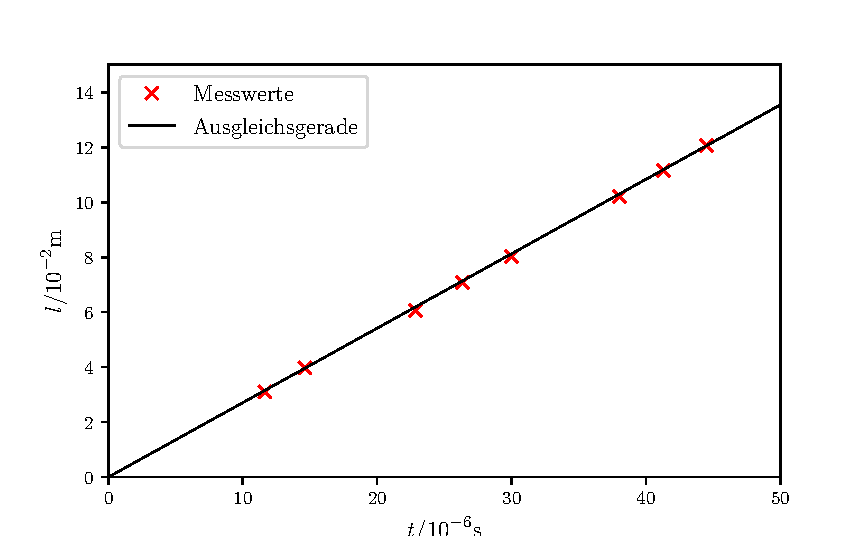
\includegraphics[width=\linewidth-70pt,height=\textheight-70pt,keepaspectratio]{content/images/Schallgeschwindigkeit.pdf}
	\label{fig:SchallIE}
\end{figure}

\noindent In der Abbildung \ref{fig:SchallIE} sind die Messwertepaare aus Tabelle \ref{tab:SchallIE} aufgetragen und durch einen linearen Fit der Form $l=c_1 t + l_{0,1}$ genähert:
\begin{align*}
	c_1&=\SI{2708(17)}{\meter\per\second}\text{,}\\
	l_{0,1}&=\SI{-6(5)e-4}{\meter}\text{.}
\end{align*}

\subsection{Bestimmung der Schallgeschwindigkeit mit Durchschallungs-Verfahren}

\begin{table}
	\centering
	\caption{Die gemessenen Zeitdifferenzen $\Delta t_.{Durchschallung}$ für die Acryl-Zylinder der Länge $l$ bei dem Durchschallungs-Verfahren.}
	\label{tab:tabSchallgeschwindigkeitDurchschallung}
	\sisetup{table-format=1.2}
	\begin{tabular}{S[table-format=2.1]S[table-format=2.2]}
		\toprule
		{$\Delta t_.{Durchschallung}/\si{\second}$} & {$l/10^{-2}\si{\metre}$} \\
		\midrule
		44.5 & 12.05 \\
		41.3 & 11.15 \\
		38.0 & 10.21 \\
		30.0 & 8.04 \\
		26.4 & 7.08 \\
		22.9 & 6.05 \\
		14.6 & 3.97 \\
		11.7 & 3.11 \\
		\bottomrule
	\end{tabular}

	\label{tab:SchallD}
\end{table}

\begin{figure}
	\centering
	\caption{Die bei einer Laufzeit $t$ zurückgelegte Strecke $l$ des Schalls im Zylinder bei dem Durchschallungs-Verfahren aufgetragen gegen die Laufzeit $t$.}
	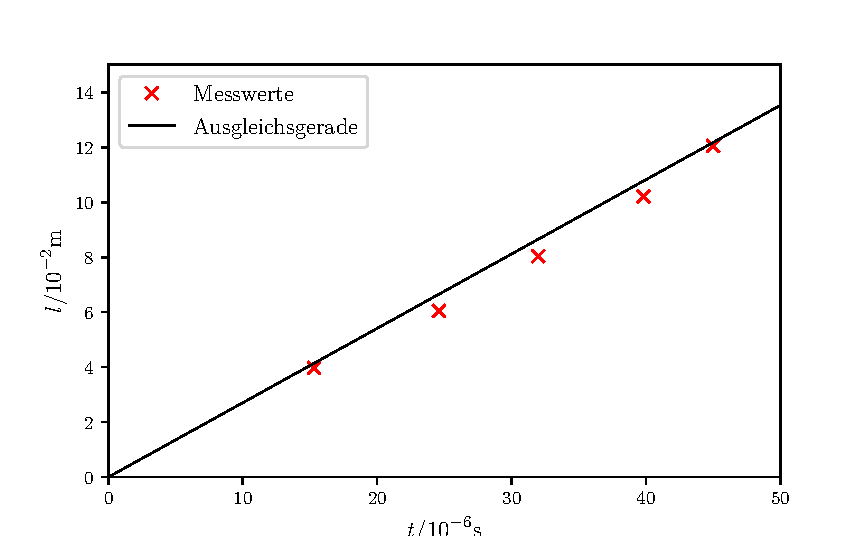
\includegraphics[width=\linewidth-70pt,height=\textheight-70pt,keepaspectratio]{content/images/SchallgeschwindigkeitDurchschallung.pdf}
	\label{fig:SchallD}
\end{figure}

\noindent In der Abbildung \ref{fig:SchallD} sind die Messwertepaare aus Tabelle \ref{tab:SchallD} aufgetragen und durch einen linearen Fit der Form $l=c_2 t + l_{0,2}$ genähert:
\begin{align*}
	c_2&=\SI{2700(120)}{\meter\per\second}\text{,}\\
	l_{0,2}&=\SI{-4(4)e-3}{\meter}\text{.}
\end{align*}

\subsection{Bestimmung der Dämpfungskonstanten mit Impuls-Echo-Verfahren}

\begin{table}
	\centering
	\caption{Die gemessene Spannungsdifferenz $\Delta U$ zur ursprünglichen Spannung für die Acryl-Zylinder der Länge $l$ bei dem Impuls-Echo-Verfahren.}
	\label{tab:tabDaempfung}
	\sisetup{table-format=1.2}
	\begin{tabular}{S[table-format=2.2]S[table-format=1.3]}
		\toprule
		{$l/10^{-2}\si{\metre}$} & {$\Delta U/\si{\volt}$} \\
		\midrule
		12.05 & 1.391 \\
		10.21 & 1.336 \\
		8.06 & 0.312 \\
		8.04 & 0.363 \\
		6.05 & 0.156 \\
		3.97 & 0.131 \\
		3.11 & 0.095 \\
		\bottomrule
	\end{tabular}

	\label{tab:Daempfung}
\end{table}

\begin{figure}
	\centering
	\caption{Der Logarithmus von den beim Impuls-Echo-Verfahren bestimmten Spannungen $U$ aufgetragen gegen die im Zylinder nach der Zeit $t$ zurückgelegte Strecke $l$ des Schalls.}
	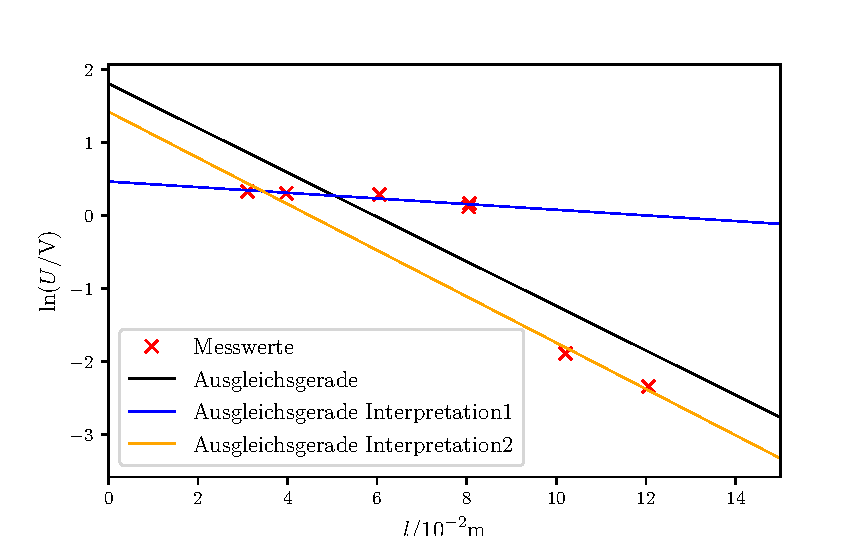
\includegraphics[width=\linewidth-70pt,height=\textheight-70pt,keepaspectratio]{content/images/Daempfung.pdf}
	\label{fig:Daempfung}
\end{figure}

\noindent In der Abbildung \ref{fig:Daempfung} ist der Logarithmus von der ursprünglichen Spannung $U$ gegen die zurückgelegte Strecke $l$ des Schalls im Zylinder mit den Werten aus Tabelle \ref{tab:Daempfung} aufgetragen und wird durch einen linearen Fit der Form $\ln(U)=-\frac{\alpha}{2} t + ln(U_0)$ genähert:
\begin{align*}
	\alpha	&= \SI{58(3)}{\per\meter}\text{,}\\
	ln(U_0)	&=\SI{1.8(7)}{\volt}\text{.}
\end{align*}
Dabei ist $\alpha$ die Dämpfung.
Aufgrund der schlechten Messwerte werden zwei weitere Näherungen derselben Form durchgeführt, einmal ohne die beiden letzten Werte (Interpretation1 in Abbildung \ref{fig:Daempfung}) und einmal ohne die drei mittleren Werte (Interpretation2 in Abbildung \ref{fig:Daempfung}). Diese liefern die Werte
\begin{align*}
	\alpha_{I1} &= \SI{8(2)}{\per\meter}\text{,}\\
	ln(U_{0,I1})&=\SI{0.47(5)}{\volt}\text{,}
\end{align*} 
für die erste Interpretation und
\begin{align*}
	\alpha_{I2} &= \SI{63(4)}{\per\meter}\text{,}\\
	ln(U_{0,I2})&=\SI{1.4(2)}{\volt}\text{,}
\end{align*}
für die zweite Interpretation.

\subsection{Untersuchung des Cepstrums/Spektrums}

\begin{table}
	\centering
	\caption{Hier Beschreibung einfügen.}
	%\input{content/images/tabCepstrum.tex}
	\label{tab:Cepstrum}
\end{table}

\noindent Im Spektrum wurde ein Peak bei $??$ aufgenommen.
Aus Tabelle \ref{tab:Cepstrum} lassen sich die Laufzeiten des Schalls in den Acrylplatten bestimmen.
Mit der bekannten Schallgeschwindigkeit in Acryl $c_.{Acryl}=\SI{2730}{\meter\per\second}$\cite{cAcryl} ergeben sich somit für die Dicken der Platten
\begin{align*}
D_1&=\SI{}{\meter}\text{,}\\
D_2&=\SI{}{\meter}\text{.}\\
\end{align*}

\subsection{Untersuchung der Abstände in einem Augenmodell}

\begin{table}
	\centering
	\caption{Die gemessenen Werte für die Laufzeiten $\Delta t_A$ des Schalls im Augenmodell.}
	\label{tab:tabAuge}
	\sisetup{table-format=1.2}
	\begin{tabular}{S[table-format=1.0]S[table-format=2.1]}
		\toprule
		{$n$} & {$\Delta t_.A/10^{-6}\si{\second}$} \\
		\midrule
		1 & 10.4 \\
		2 & 16.2 \\
		3 & 23.3 \\
		4 & 31.6 \\
		5 & 73.4 \\
		\bottomrule
	\end{tabular}

	\label{tab:Auge}
\end{table}

\noindent Mit den Werten für die Laufzeiten des Schalls im Auge aus Tabelle \ref{tab:Auge} lässt sich mit den bekannten Schallgeschwindigkeiten von $c_.{GK}=\SI{1410}{\meter\per\second}$ außerhalb der Linse und von $c_.{L}=\SI{2500}{\meter\per\second}$ in der Linse die Abstände im Augenmodell berechnen. Für den Abstand zwischen der Hornhaut und der Iris ergibt sich
\begin{equation*}
A_1=\SI{}{\meter}\text{,}
\end{equation*}
für den Abstand zwischen Iris und Linse
\begin{equation*}
A_2==\SI{}{\meter}\text{,}
\end{equation*}
für die Dicke der Linse
\begin{equation*}
A_3=\SI{}{\meter}
\end{equation*}
und für den Abstand zwischen Linse und Retina 
\begin{equation*}
A_4=\SI{}{\meter}\text{.}
\end{equation*}